\documentclass[12pt]{exam}
\usepackage{amsmath}
\usepackage{amssymb}
\usepackage{amsthm}
\usepackage{tikz}
\usepackage{mathtools}
\usepackage{graphicx}
\usepackage{wrapfig}

\usepackage{bm} %bold symbols
\usepackage{hyperref} %add links

%%%%%%%%%%%%%%%%%%%%%%%%%
% 	Define vars here 	%
%%%%%%%%%%%%%%%%%%%%%%%%%

\def\hwName{Homework Set 4: §14.1 – 14.5}
\author{Zhengyu James Pan} %use like \@author
\def\email{jzpan@umich.edu}
\makeatletter

\begin{document}
%Header
\pagestyle{head}
\firstpageheader{}{}{}
\header{MATH 215}{\hwName}{\thepage}

%Solution formatting
\printanswers
\unframedsolutions

%Top matter
{\parindent0in
\begin{center}
	\bf MATH 215 FALL 2023\\
	\bf \hwName \\
	\@author\ (\href{mailto:\email}{\email})
\end{center}
}

\begin{questions}
%1
\question Do Exercise 32 of §14.1 of Stewart’s Multivariable Calculus.
%\clearpage
%2
\question Do Exercises 61-66 of §14.1 of Stewart’s Multivariable Calculus.
%\clearpage
%3
\question Do Exercise 6 of §14.3 of Stewart’s Multivariable Calculus.
%\clearpage
%4
\question 
	\begin{parts}
		\part Suppose $g(x, y) = \sqrt{9 - 9x^2 - y^2}$. Draw a contour map for g and then sketch the graph of $g$.
		\part Draw a contour map of the function $m(x, y) = \frac{x}{(x2 + 3y2)}$, showing and labelling several level curves.
		curves.
	\end{parts}
%5
\question 
	\begin{parts}
		\part Use a linear approximation to estimate $(0.99)3 + (2.01)3 - 6(0.99)(2.01)$.
		\part Let $f(x, y) = xe^{y^2} - ye^{x^2}$ and find the equation for the tangent plane to the graph of $f$ at (1, 2).
		\part What point on the surface $z = x^2 - y^2$ has a tangent plane parallel to the plane found in the previous part?
	\end{parts}
%6
\question The wave heights h in the open sea depend on the speed $v$ of the wind and the length of time $t$ that the wind has been blowing at that speed. Values of the function $h = f (v, t)$ are recorded in feet in the following table:
	\begin{center}
		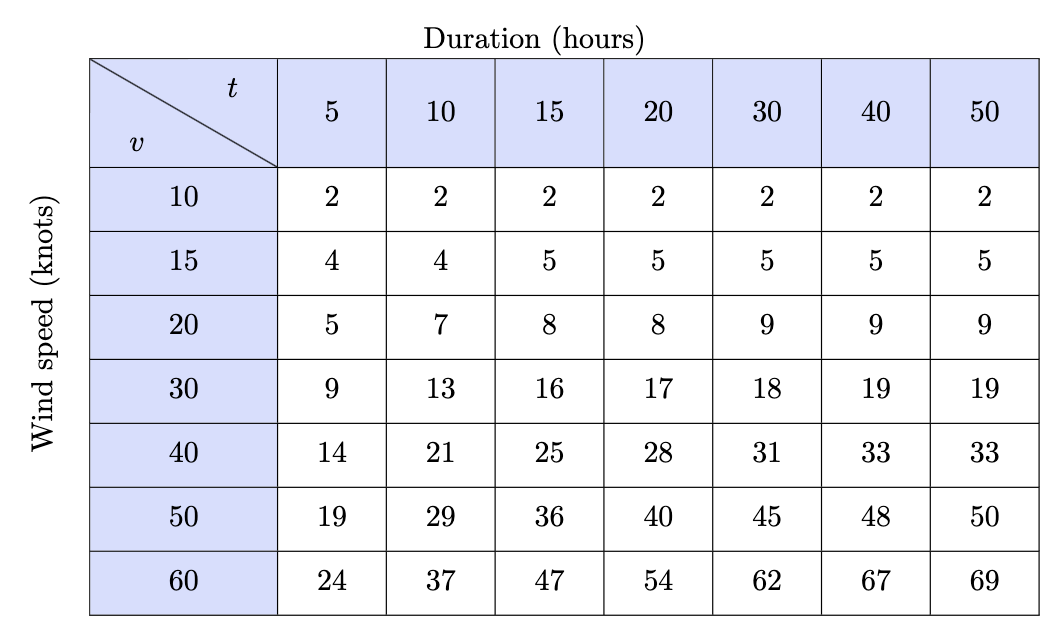
\includegraphics[scale = 0.8]{images/04-table.png}
	\end{center}
	\begin{parts}
		\part What are the meanings of the partial derivatives $\frac{\delta h}{\delta v}$ and $\frac{\delta h}{\delta t}$?
		\part Estimate the values of $f_v (40, 15)$ and $f_t(40, 15)$. What are the practical interpretations of these values?
		\part Estimate the values of $f_{vv} (30, 20), f_{tt}(30, 20), f_{vt}(30, 20)$, and $f_{tv} (30, 20)$. Are your answers for $f_{tv}$
		the same as for $f_{vt}$? Should they be? Explain. Hint: This problem might be trickier than it looks.
	\end{parts}
%7
\question Determine which of the following functions is a solution to Laplace’s equation uxx + uyy = 0:
	\begin{parts}
		\part 
	\end{parts}
\end{questions}

\end{document}